\documentclass[11pt,a4paper]{article}
\usepackage{url,hyperref,lineno,microtype,subcaption}
\usepackage{color,tensor,multirow,siunitx}
\usepackage[onehalfspacing]{setspace}
\usepackage{makecell}
\renewcommand{\cellalign}{cl}
\renewcommand{\rmdefault}{phv}
\usepackage{graphicx}
\usepackage{caption}
\captionsetup[figure]{name=Fig., labelfont=bf}

\renewcommand{\cellalign}{cl}

\newcommand{\ds}{\displaystyle}
\newcommand{\nl}{\ \\ }
\newcommand{\ud}{\textrm{ d}}
\newcommand{\bs}{\bigskip}

\newcommand{\bu}{\mathbf{u}}
\newcommand{\bv}{\mathbf{v}}
\newcommand{\bx}{\mathbf{x}}
\newcommand{\be}{\mathbf{e}}
\newcommand{\bb}{\mathbf{b}}
\newcommand{\bk}{\mathbf{k}}
\newcommand{\bn}{\mathbf{n}}
\newcommand{\bR}{\mathbf{R}}

\definecolor{red}{rgb}{1,0,0}
\definecolor{blue}{rgb}{0,0,0.8}
\definecolor{green}{rgb}{0,0.5,0}
\newcommand{\emphc}[1]{\emph{\textcolor{red}{#1}}}
\newcommand{\modif}[1]{\textcolor{red}{#1}}
\newcommand{\hycom}{\textsc{hycom} }
\newcommand{\slim}{\textsc{slim}\ }
\newcommand{\ie}{{\it i.e.}\ }
\newcommand{\eg}{{\it e.g.}\ }
\newcommand{\edit}[1]{\textcolor{orange}{#1}}
\linenumbers


\title{Some nice title}
\author{Thomas Dobbelaere, Emmanuel Hanert (and other co-authors to be determined)}

\begin{document}

\maketitle
\begin{abstract}
Some nice abstract
\end{abstract}

% === INTRODUCTION === %
\section{Introduction}


% === METHODS === %
\section{Methods}
\subsection{Wind and atmospheric pressure for Hurricane Irma}
\subsection{Hydrodynamic model}
\begin{figure}
    \centering
    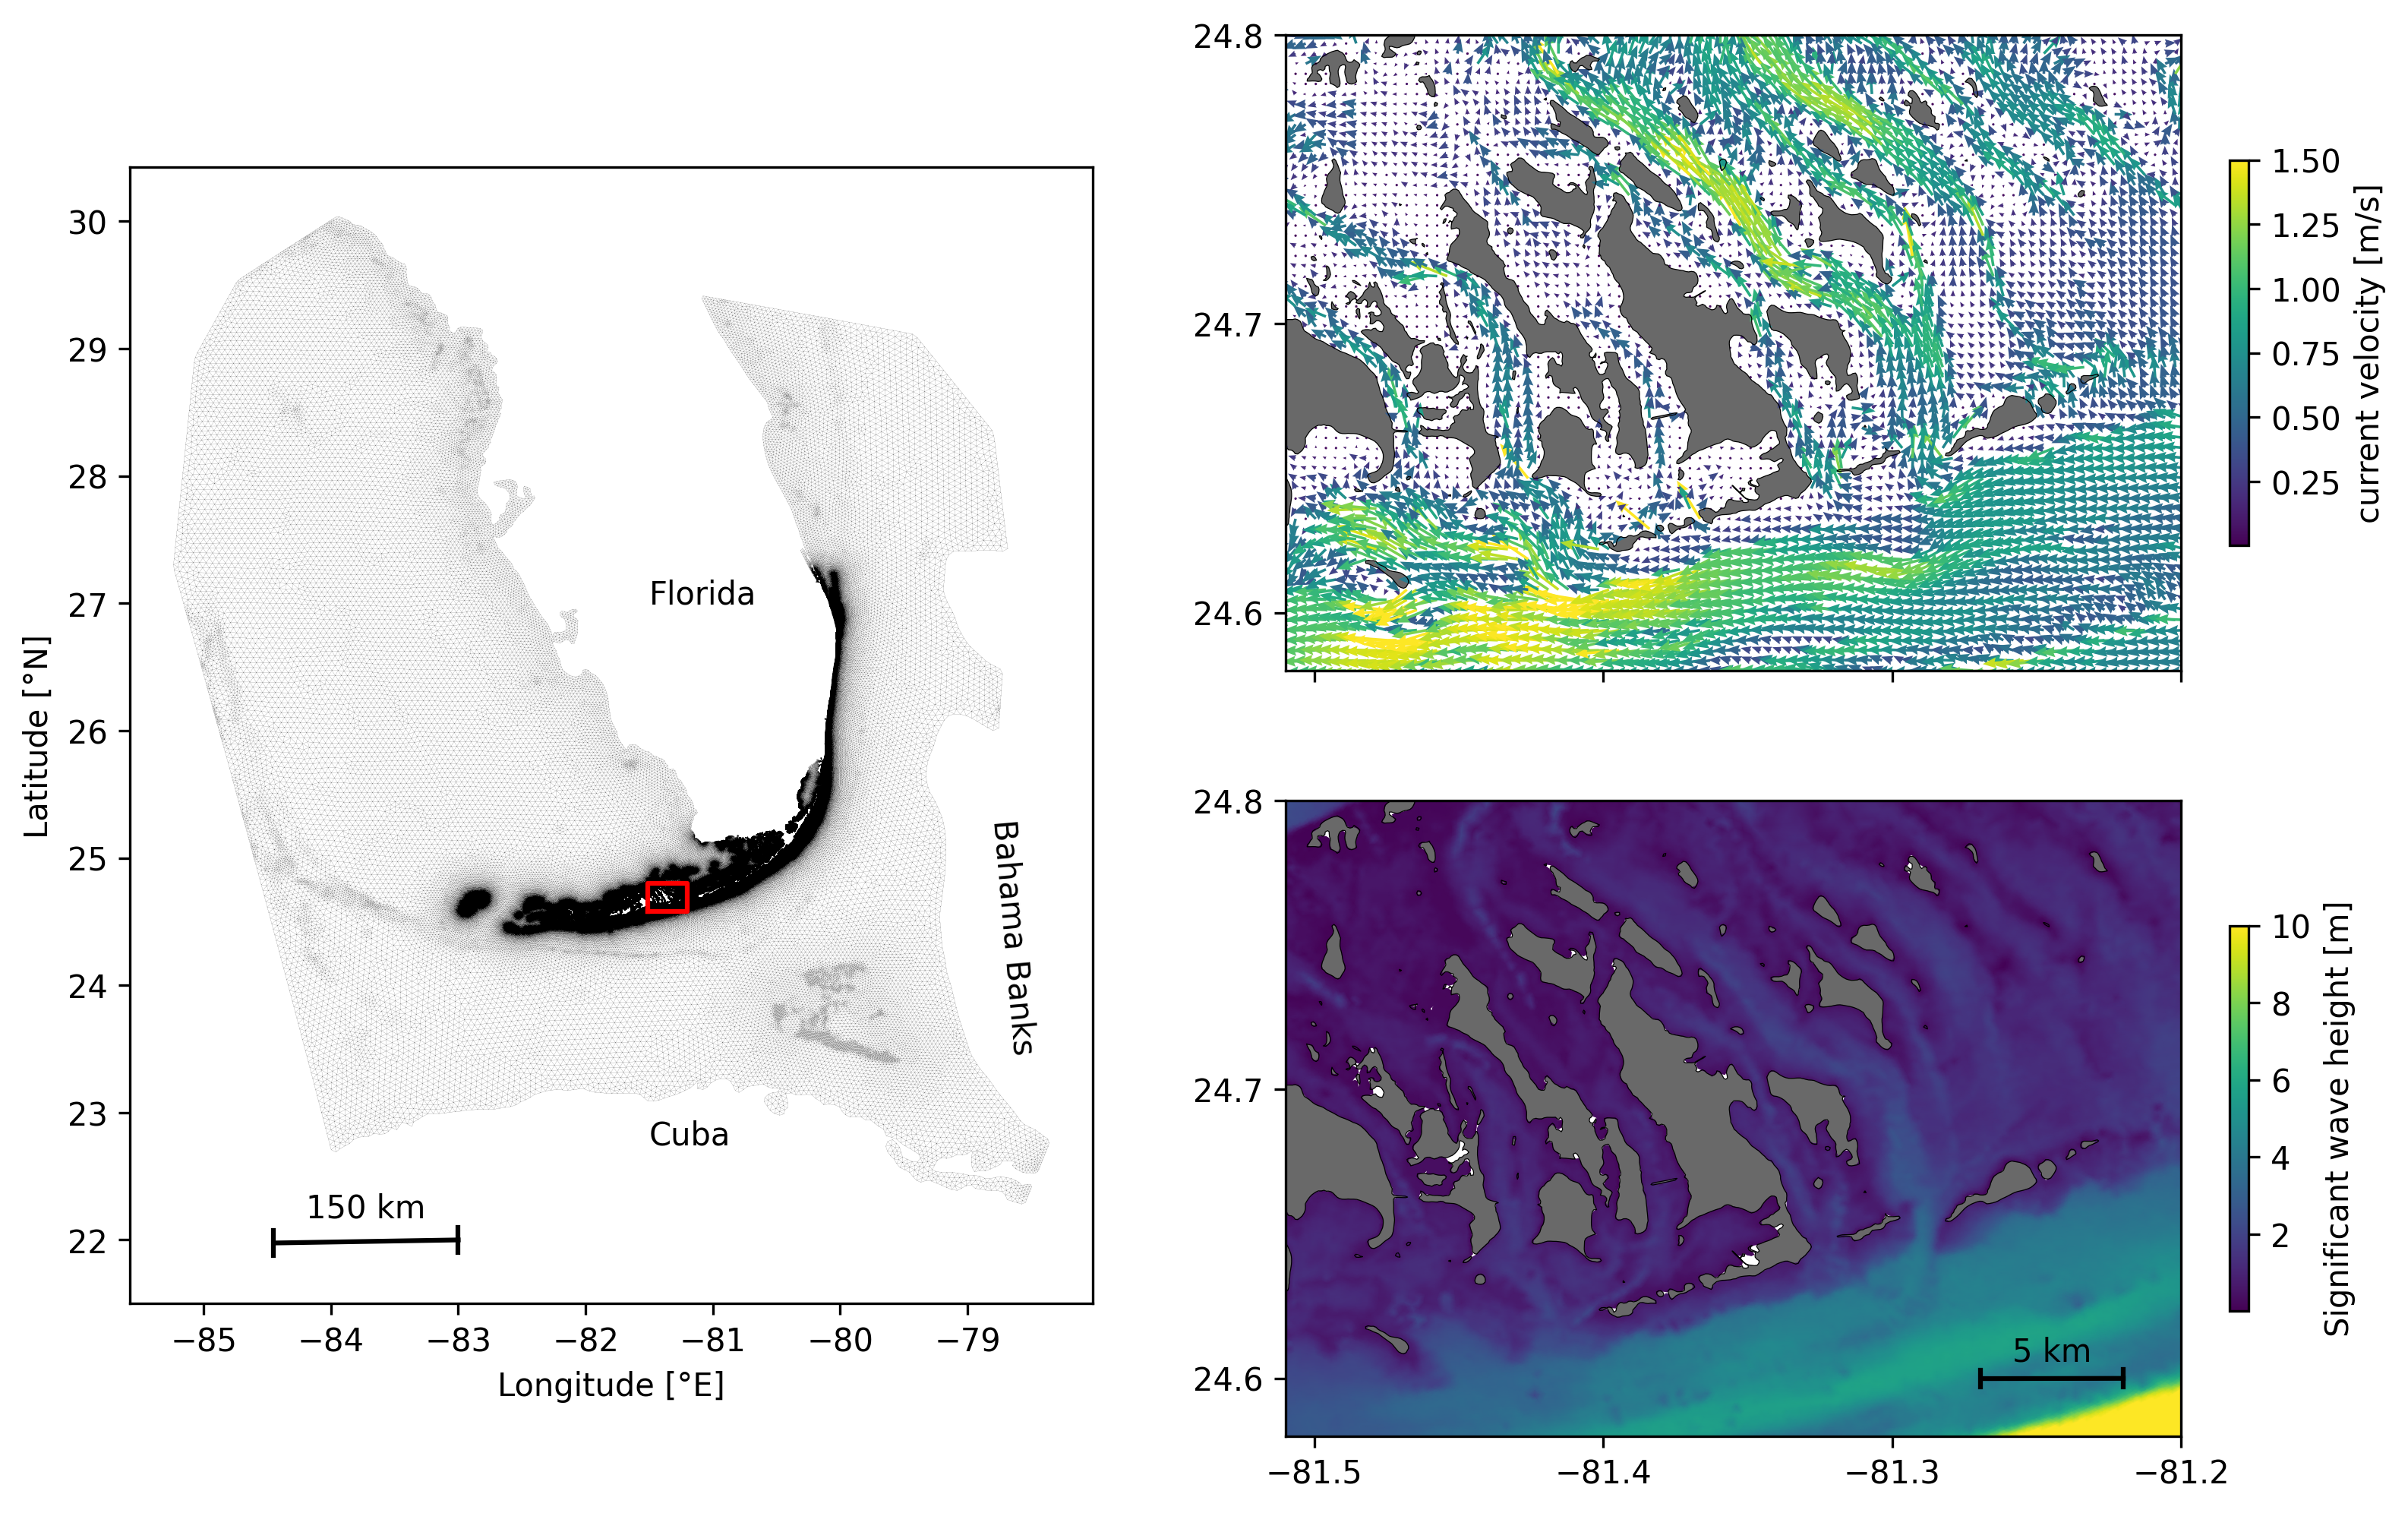
\includegraphics[width=.95\textwidth]{fig/fig_mesh_ww3.png}
    \caption{Mesh of the computational domain with snapshots of simulated instantaneous currents and significant wave height on 2017-09-10 at 11:00:00. The mesh resolution ranges from 100 m in the Florida Keys to a maximum of 10 km offshore.}
    \label{fig:mesh}
\end{figure}
\subsection{Wave model}
\subsection{Coupled model}

%%%%%%%%%%%%%%%%%%%
% --- RESULTS --- %
%%%%%%%%%%%%%%%%%%%
\section{Results}

\subsection{Validation}
\begin{figure}
    \centering
    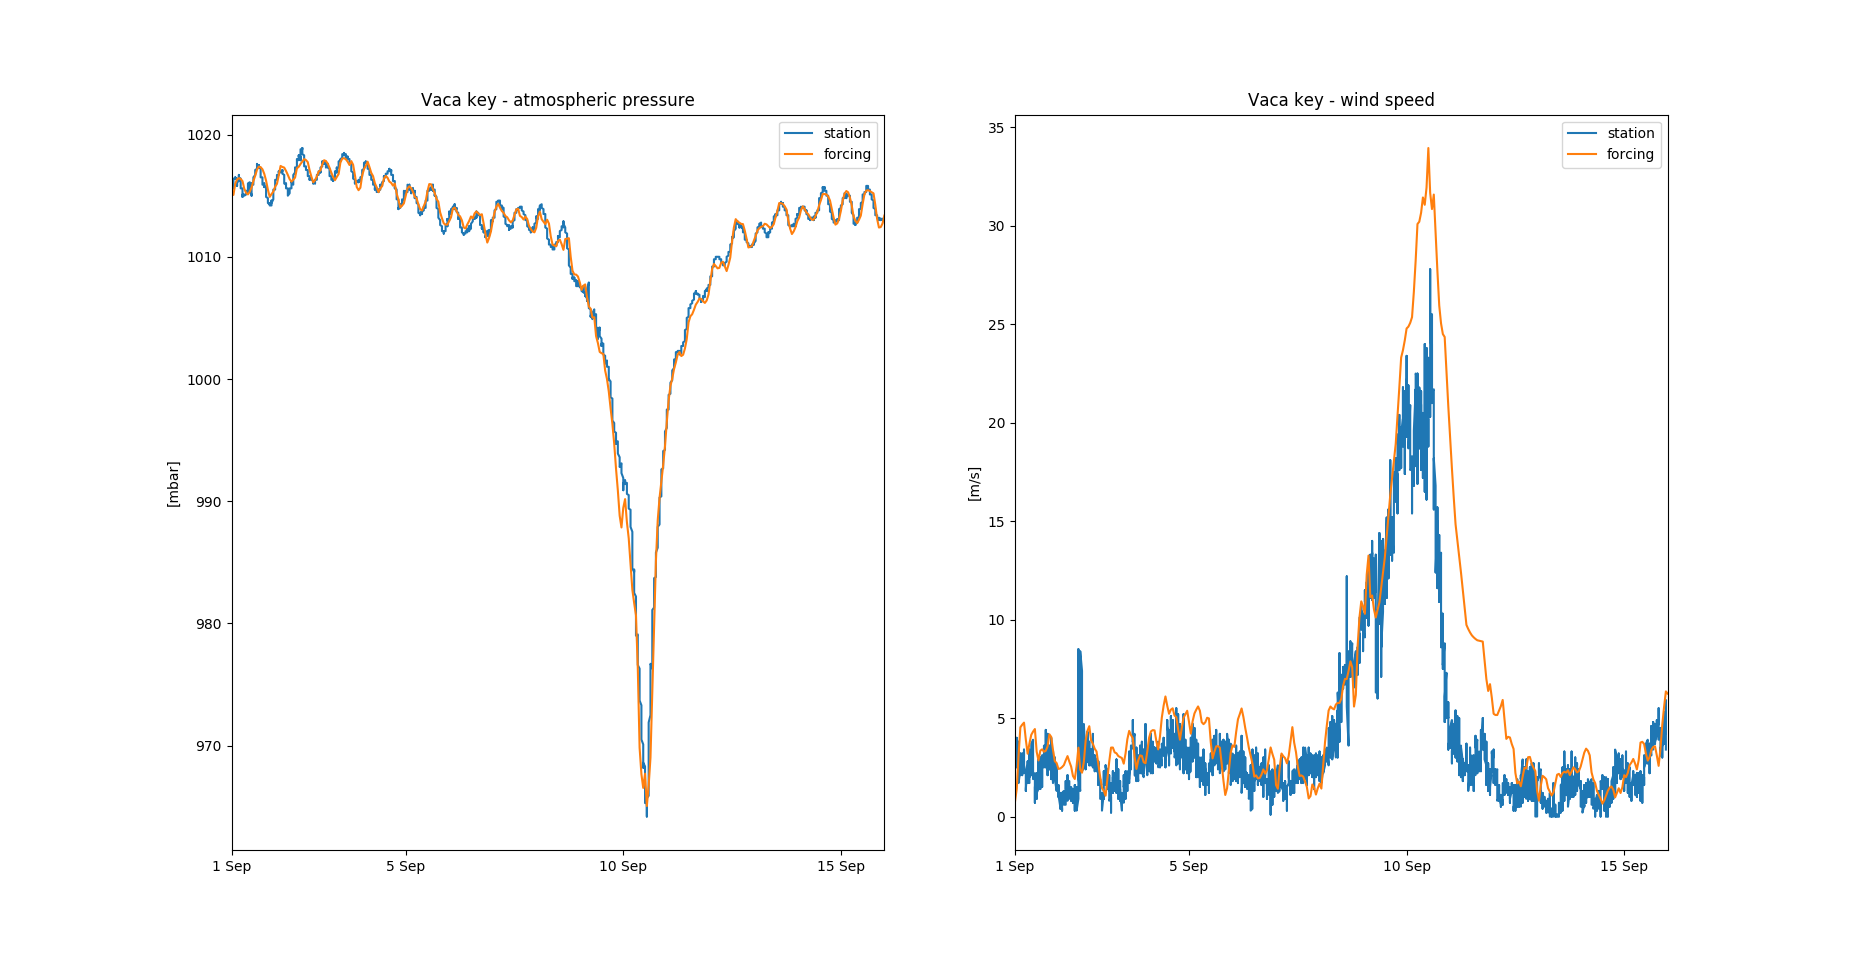
\includegraphics[width=.95\textwidth]{fig/validation_met.png}
    \caption{The atmospheric forcings have been validated with meteorological station observations at Vaca Key. The reconstructed atmospheric pressure and wind speed agree well with field measurements.}
    \label{fig:forcings}
\end{figure}

\begin{figure}
    \centering
    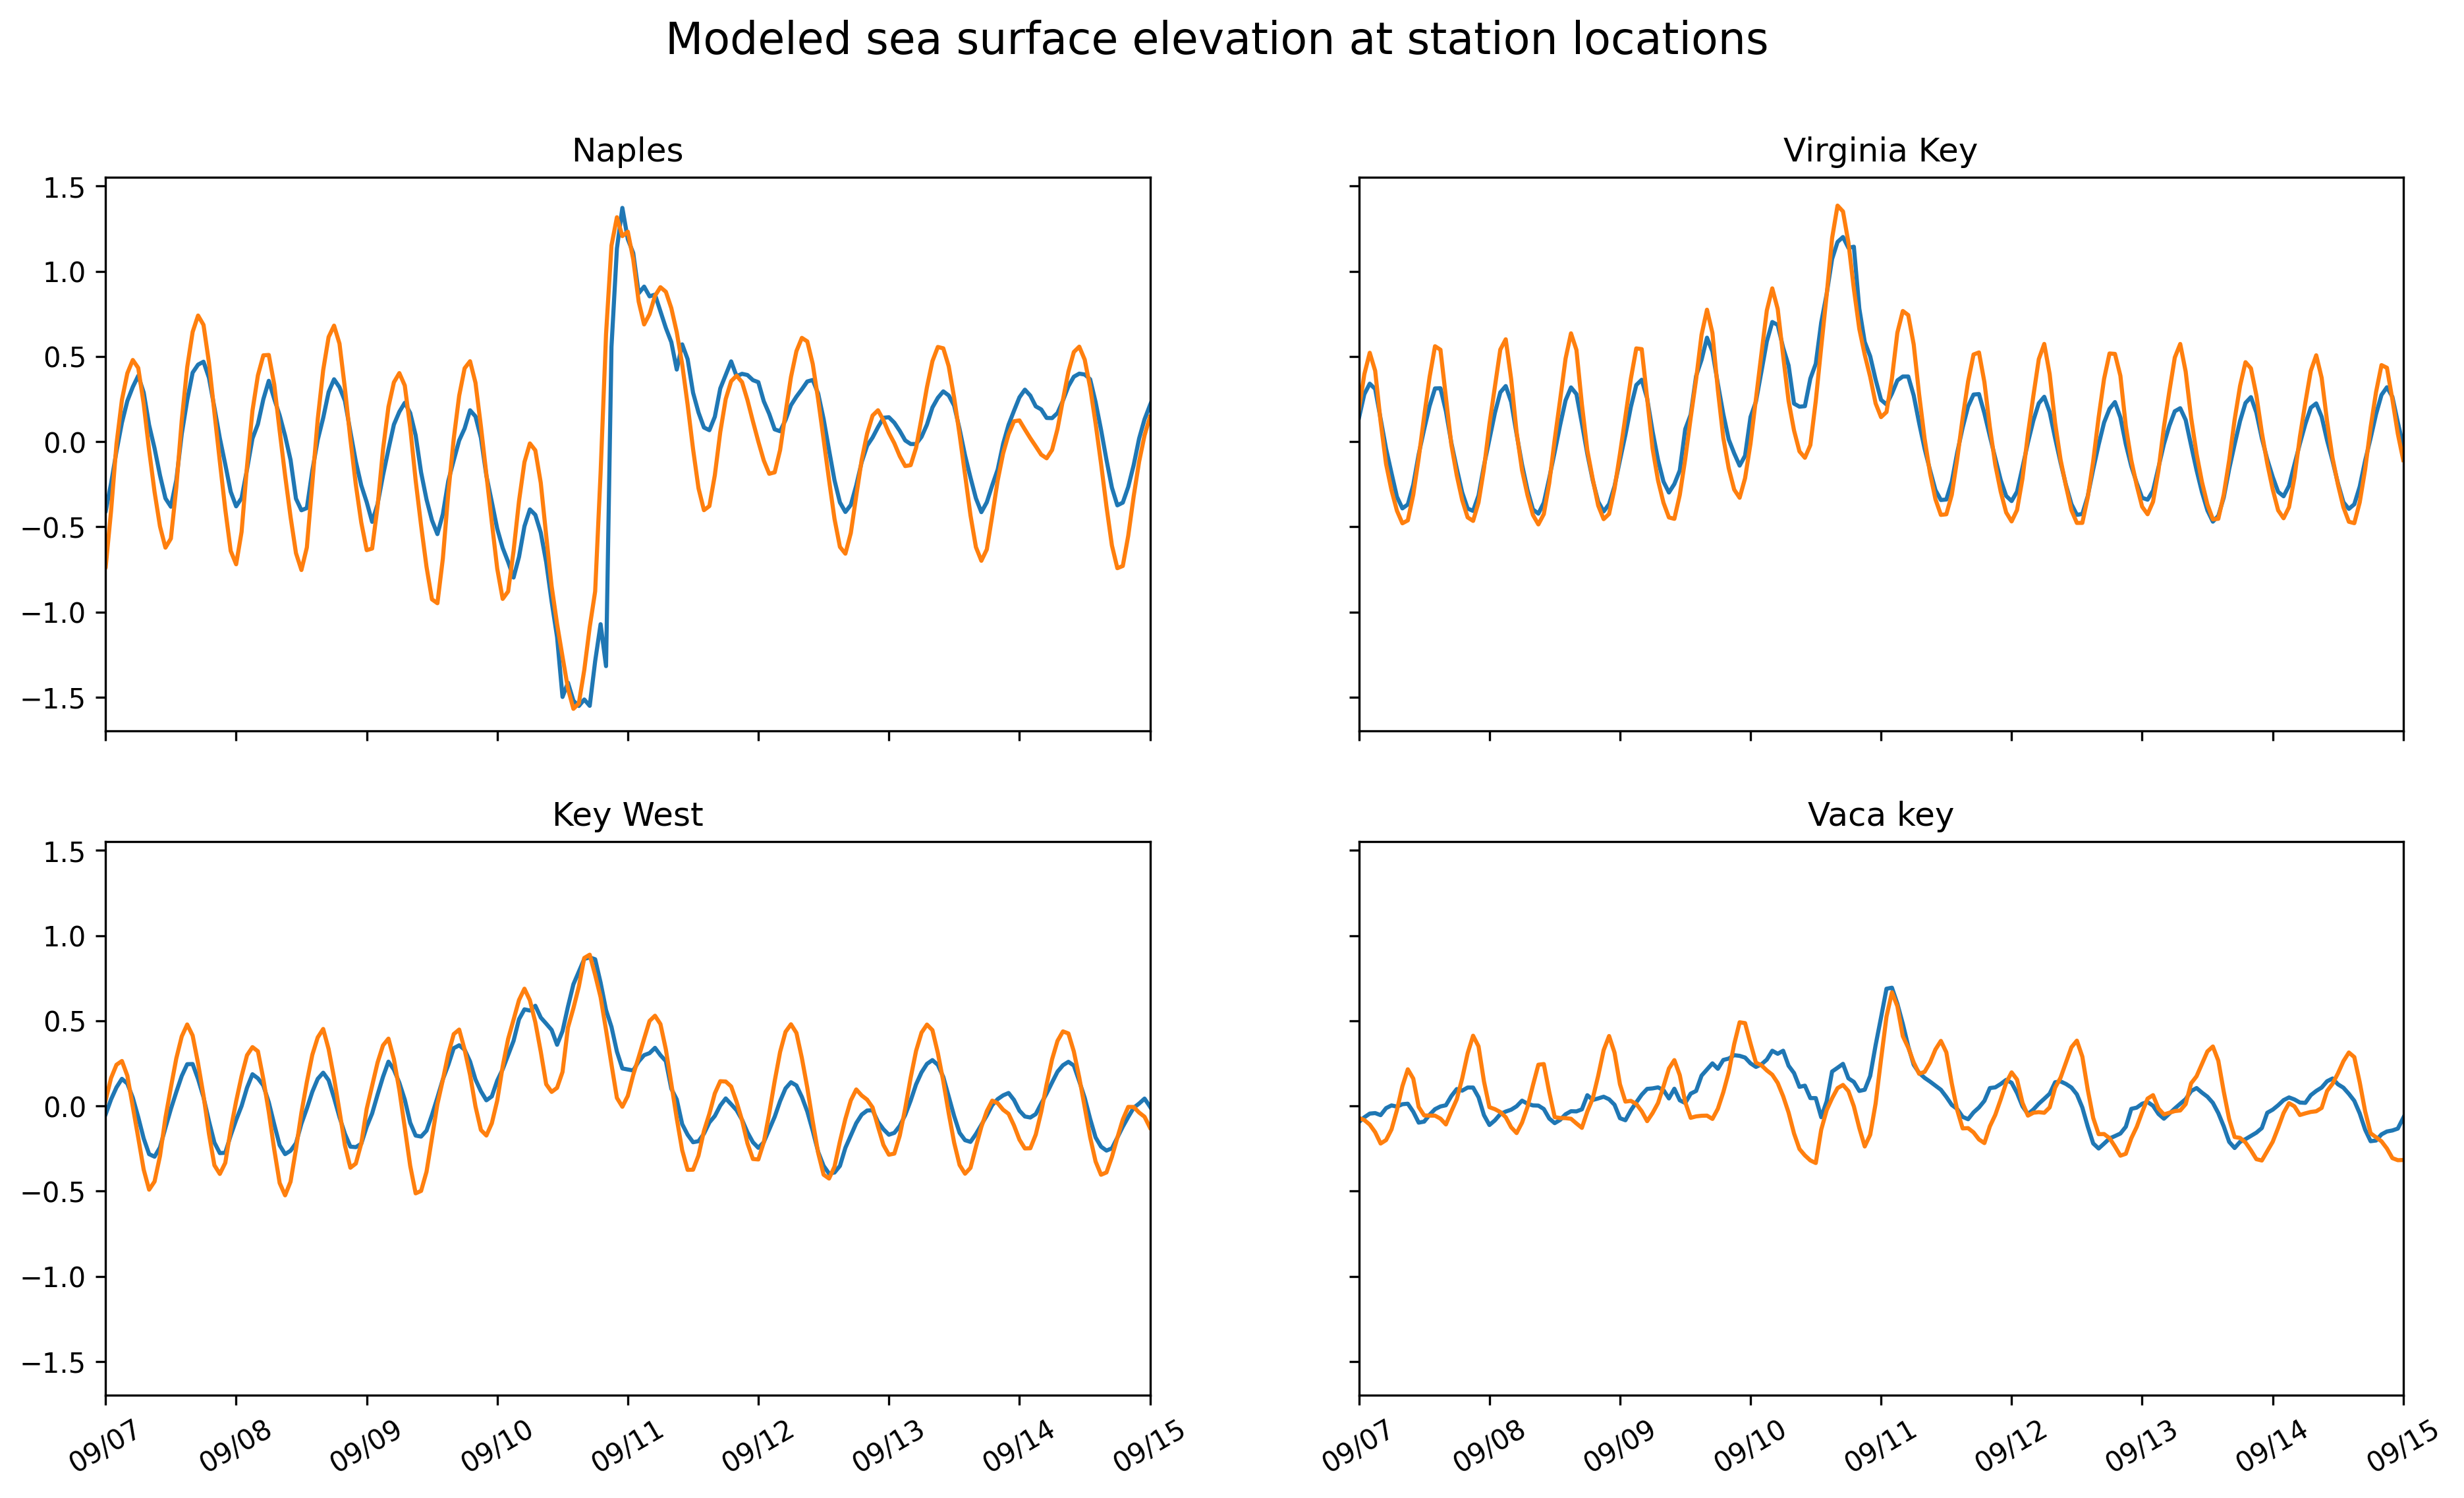
\includegraphics[width=.95\textwidth]{fig/elevation_with_map.png}
    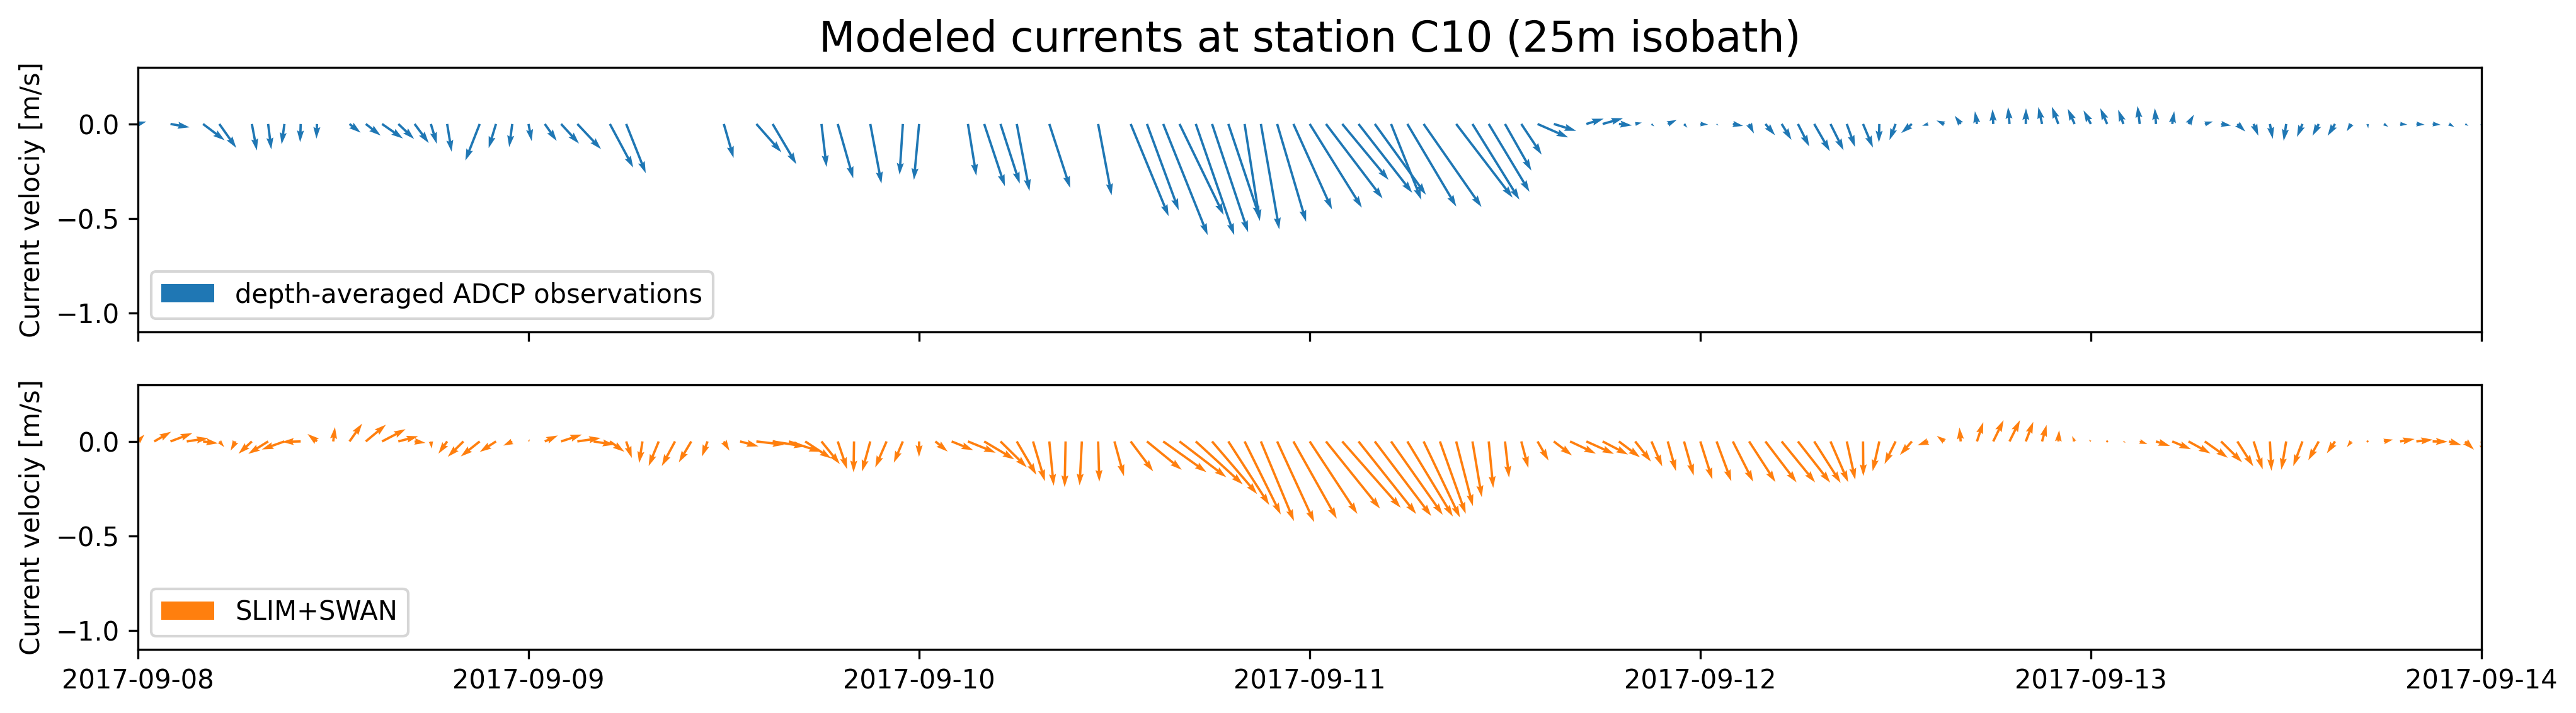
\includegraphics[width=.95\textwidth]{fig/validation_currents_C10_ww3.png}
    \caption{The sea-surface elevation produced by the coupled wave-current model agrees with SSE and current velocity observations at different stations. The fit is particularly good in the Florida Keys and in Naples, on the inner Florida shelf. The coupled model currents have been validated against current meter data on the inner Florida shelf. The current speed and direction during the hurricane agrees well with the observations.}
    \label{fig:hydro}
\end{figure}

\begin{figure}
    \centering
    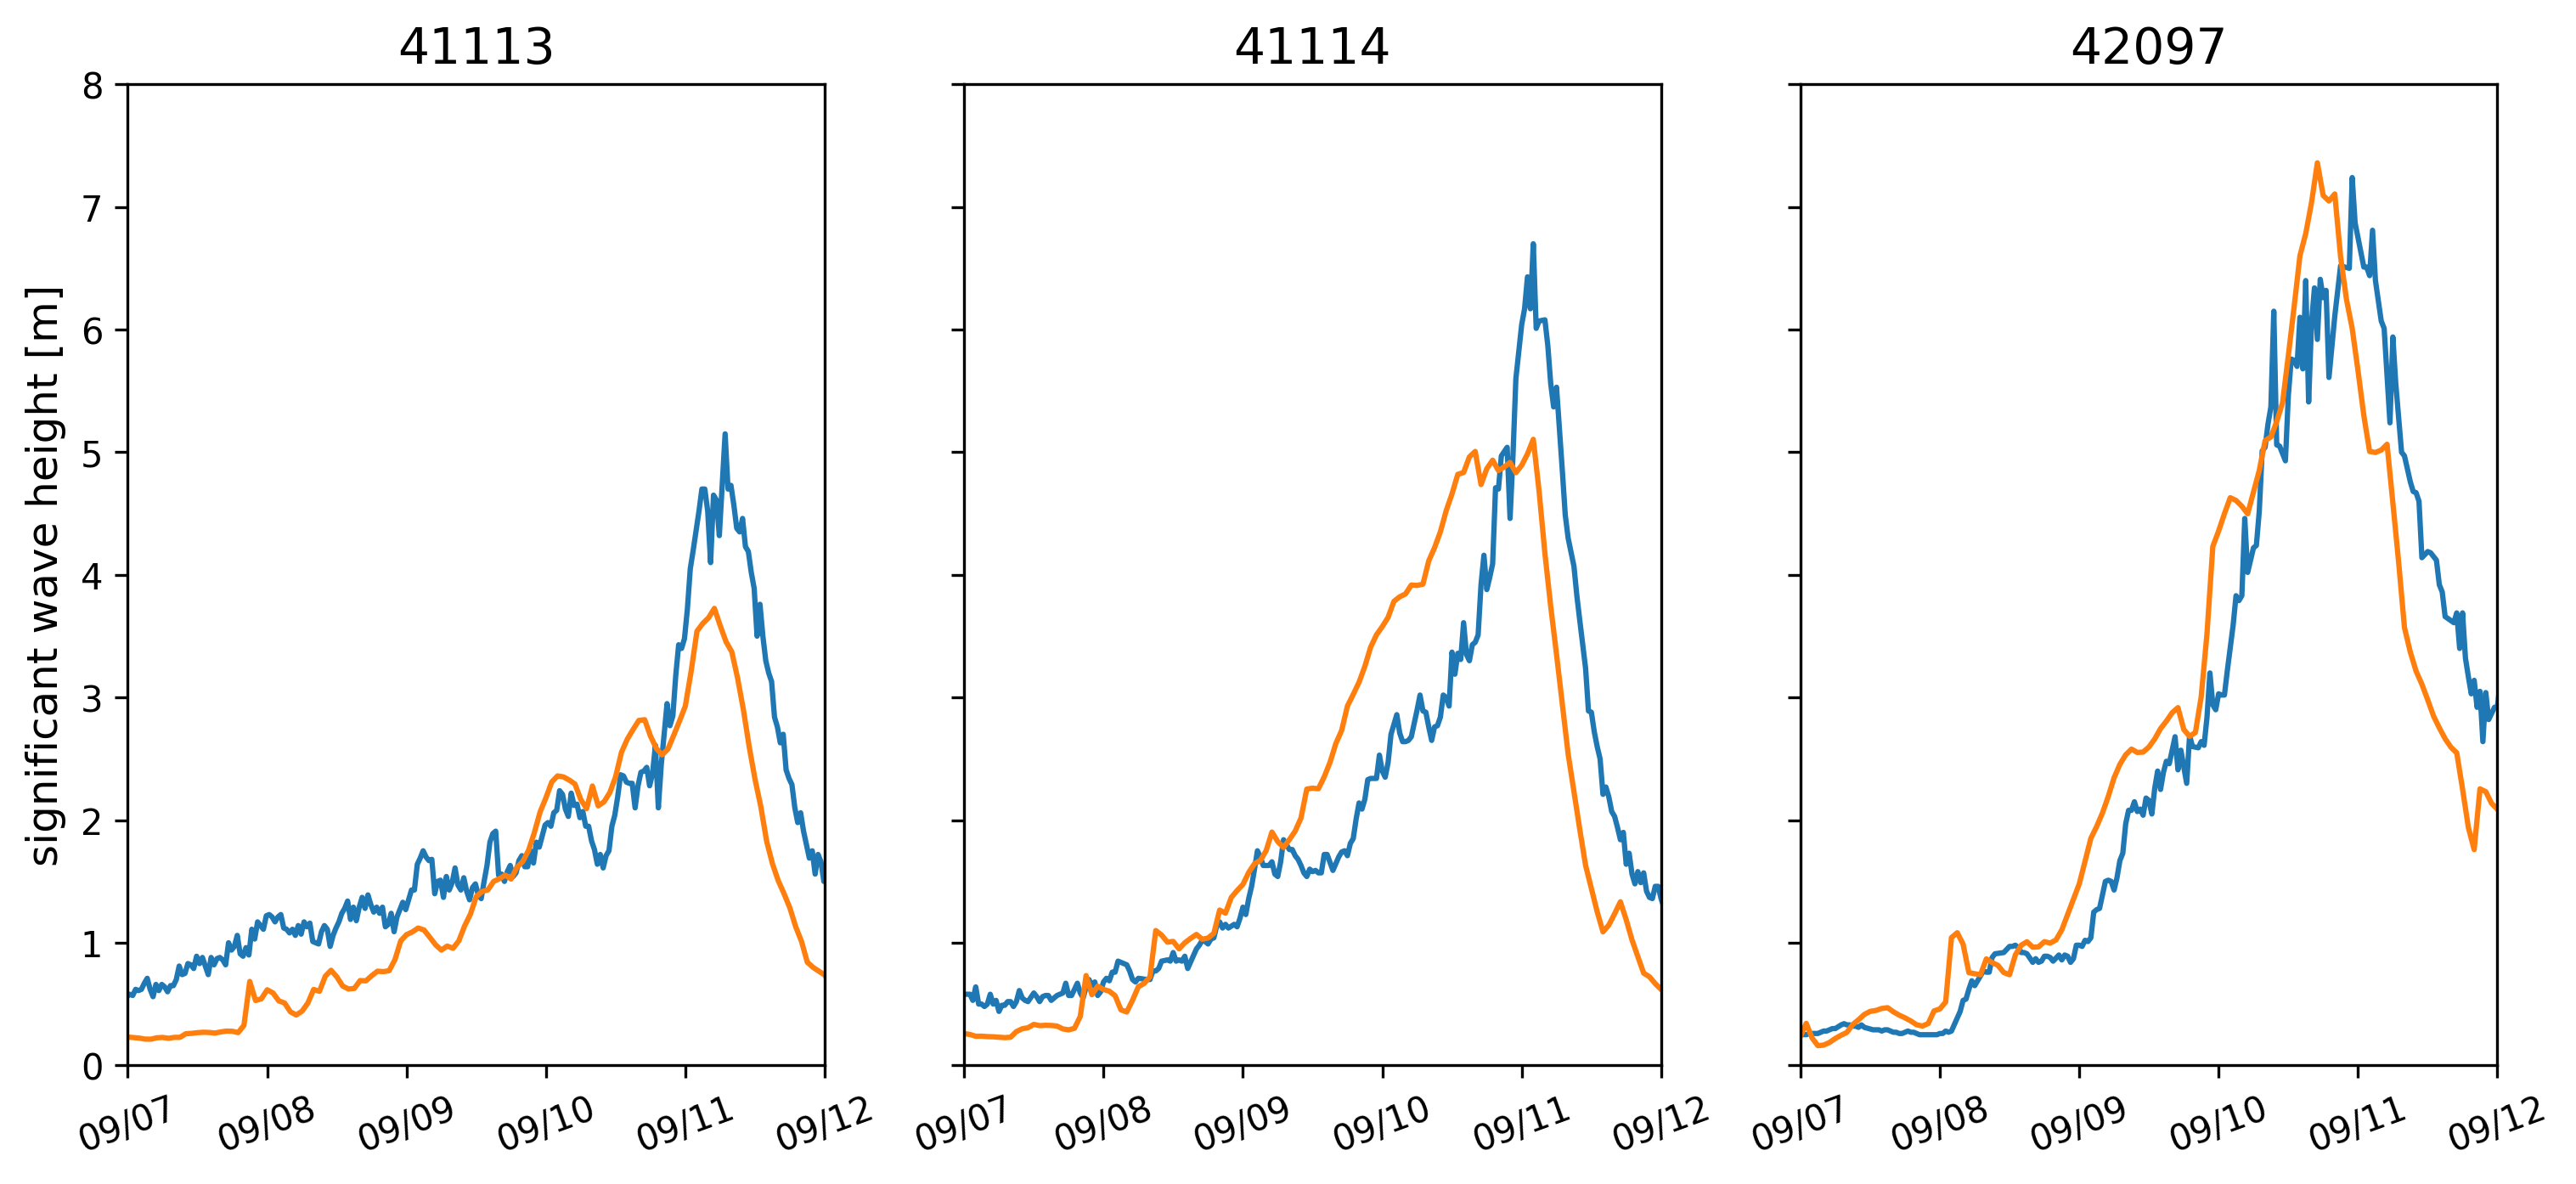
\includegraphics[width=.95\textwidth]{fig/hsig_with_map_ww3.png}
    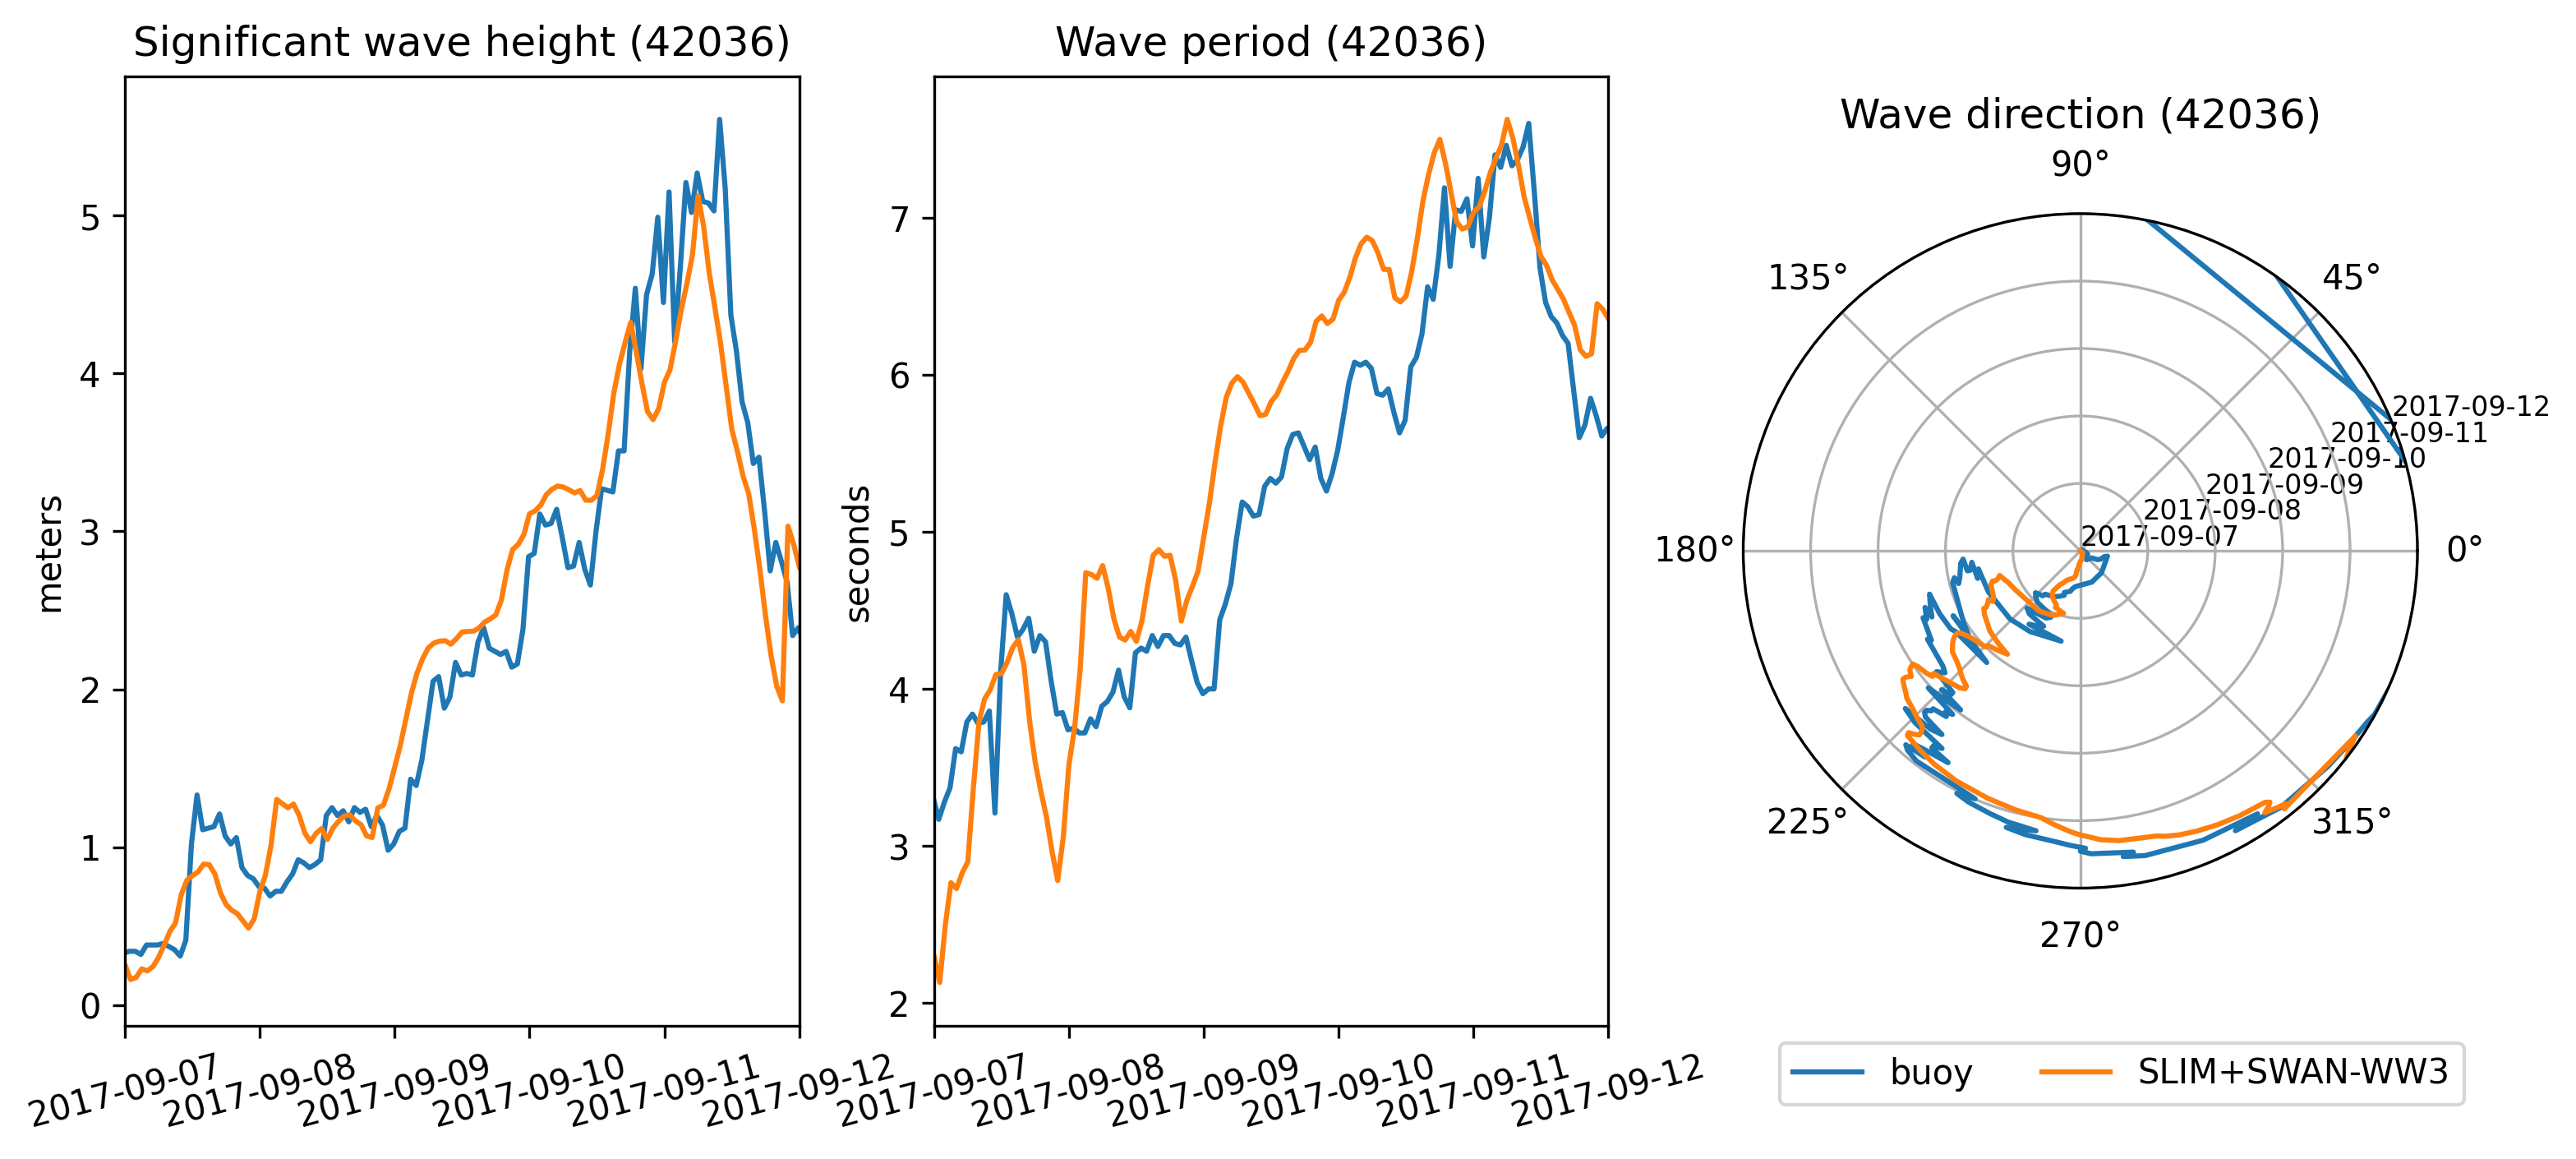
\includegraphics[width=.95\textwidth]{fig/val_waves.png}
    \caption{The significant wave height produced by the coupled model has been compared to buoy measurements at 4 different stations. The timing and amplitude of the peak during the hurricane is correctly reproduced for all stations. For station 42036, the period and direction of the waves also agree well with observations}
    \label{fig:waves}
\end{figure}

\subsection{Impact of waves}

\begin{figure}
    % TODO: Islands in Grey
    \centering
    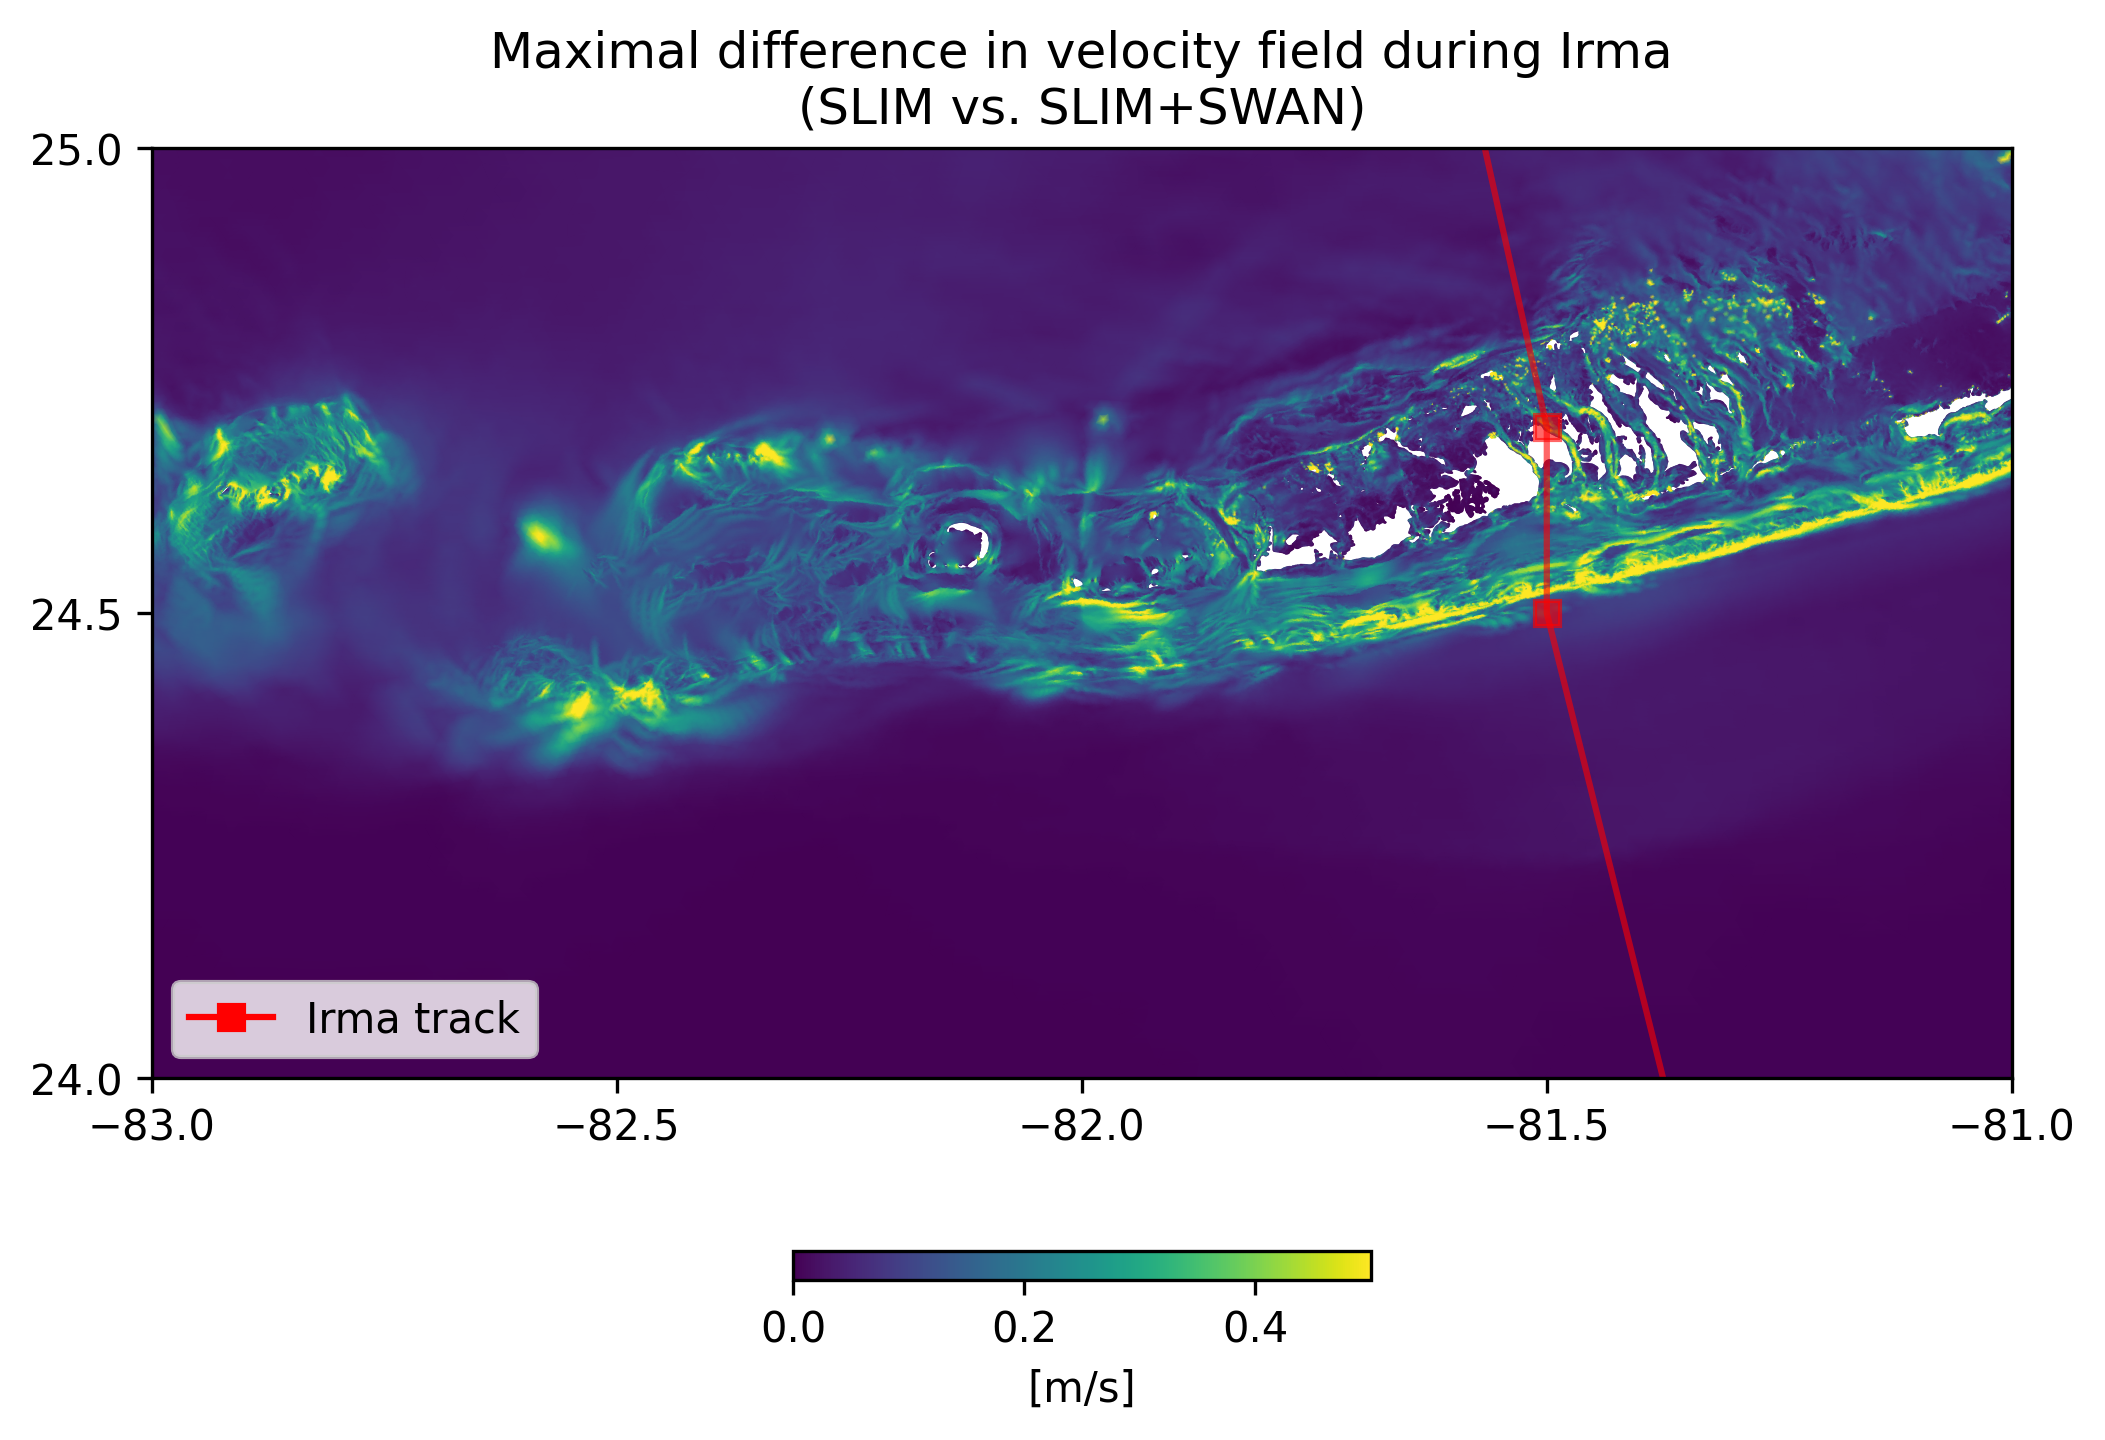
\includegraphics[width=.95\textwidth]{fig/max_diff_ww3.png}
    \caption{Maximum of the difference between SLIM and SLIM+SWAN currents speed between 2017-09-07 00:00:00 and 2017-09-13 00:00:00. The difference between the coupled and uncoupled model, which represents the effect of the wave-induced stress, can yield differences of 0.5 m/s in the simulated currents during the passage of the hurricane. SLIM+SWAN currents velocities are larger than the currents modeled by SLIM alone.}
    \label{fig:diff}
\end{figure}

\begin{figure}
    \centering
    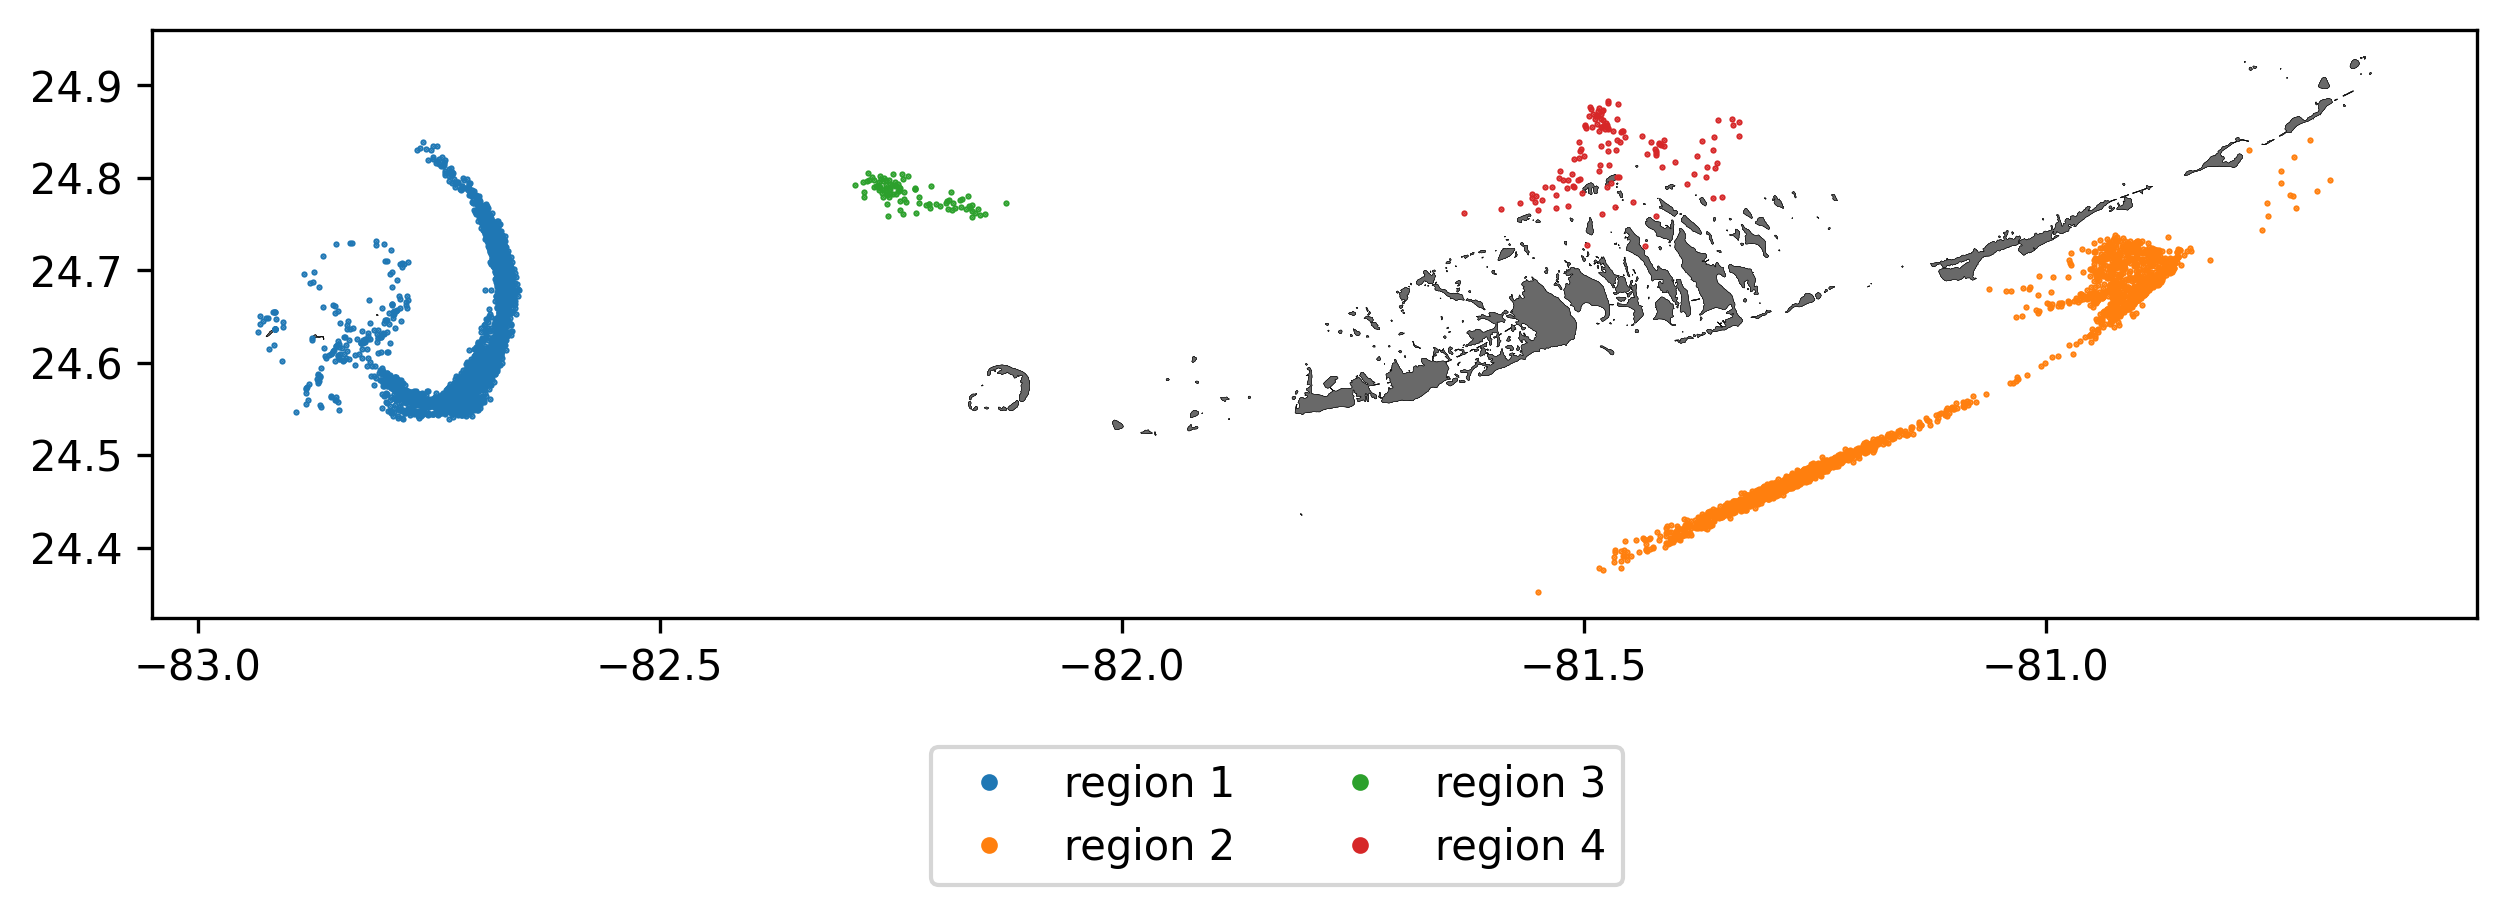
\includegraphics[width=.75\textwidth]{fig/release_regions.png}
    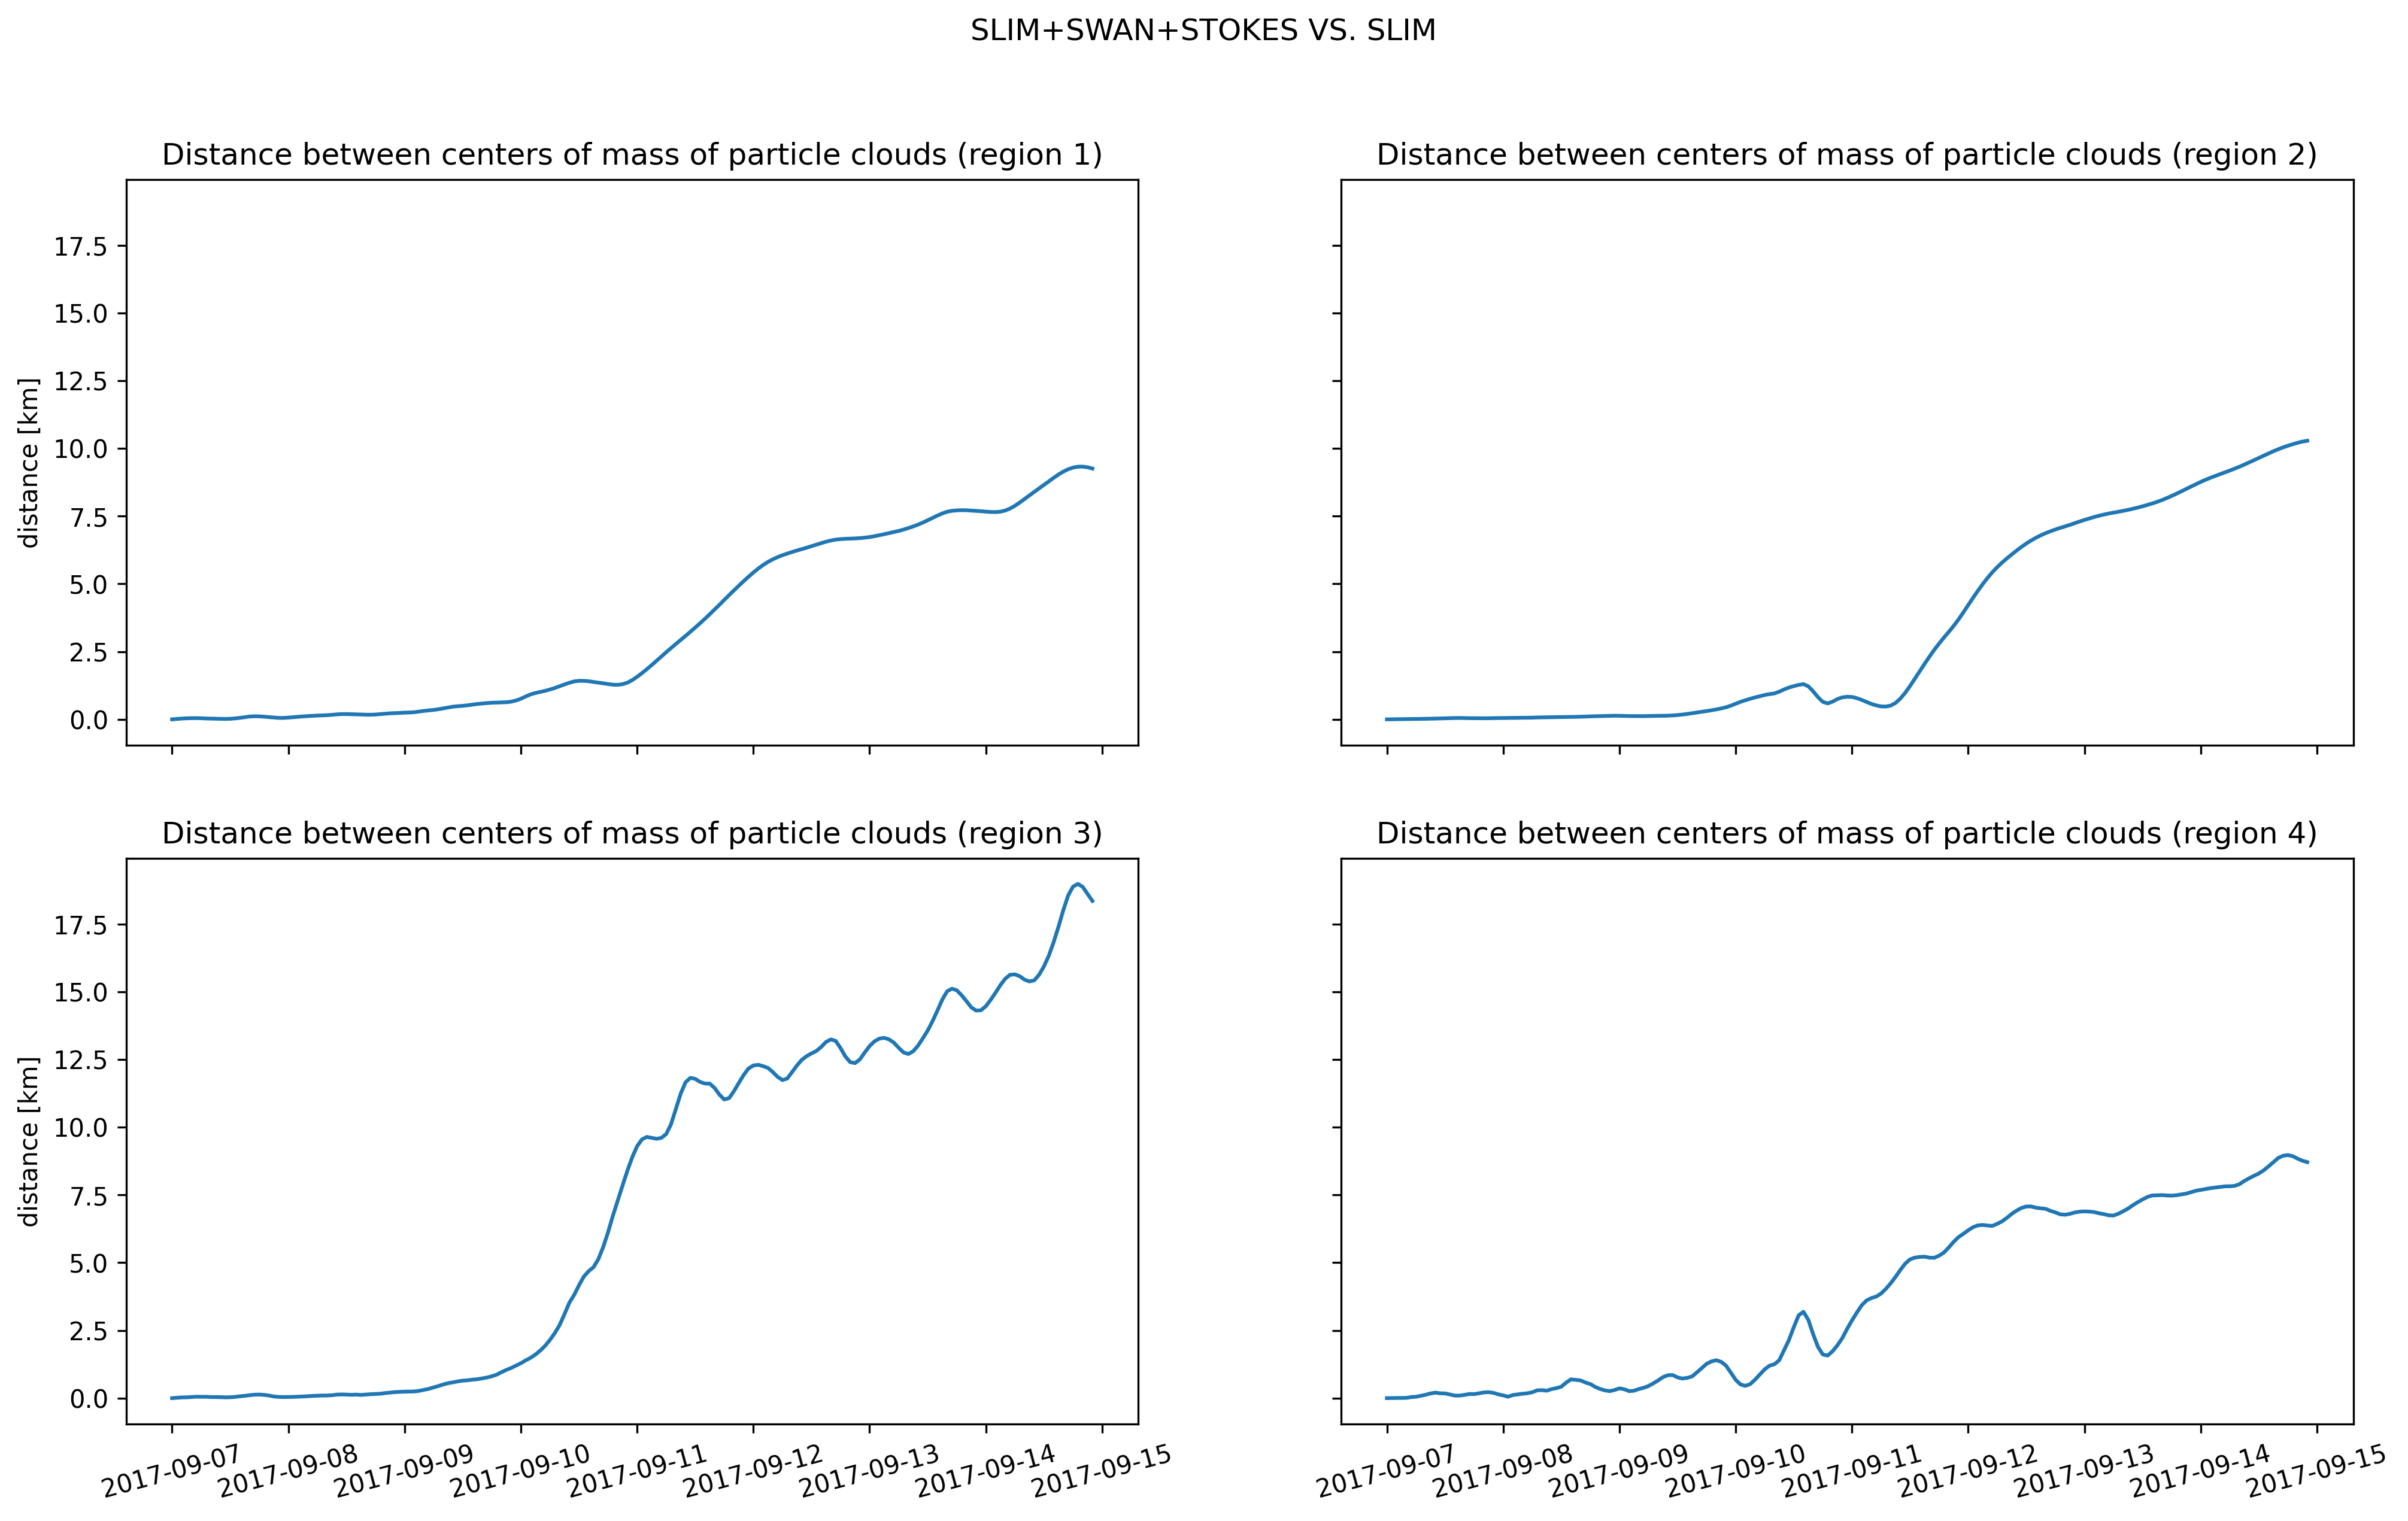
\includegraphics[width=.95\textwidth]{fig/slim+swan+stokes_vs_slim_WW3.png}
    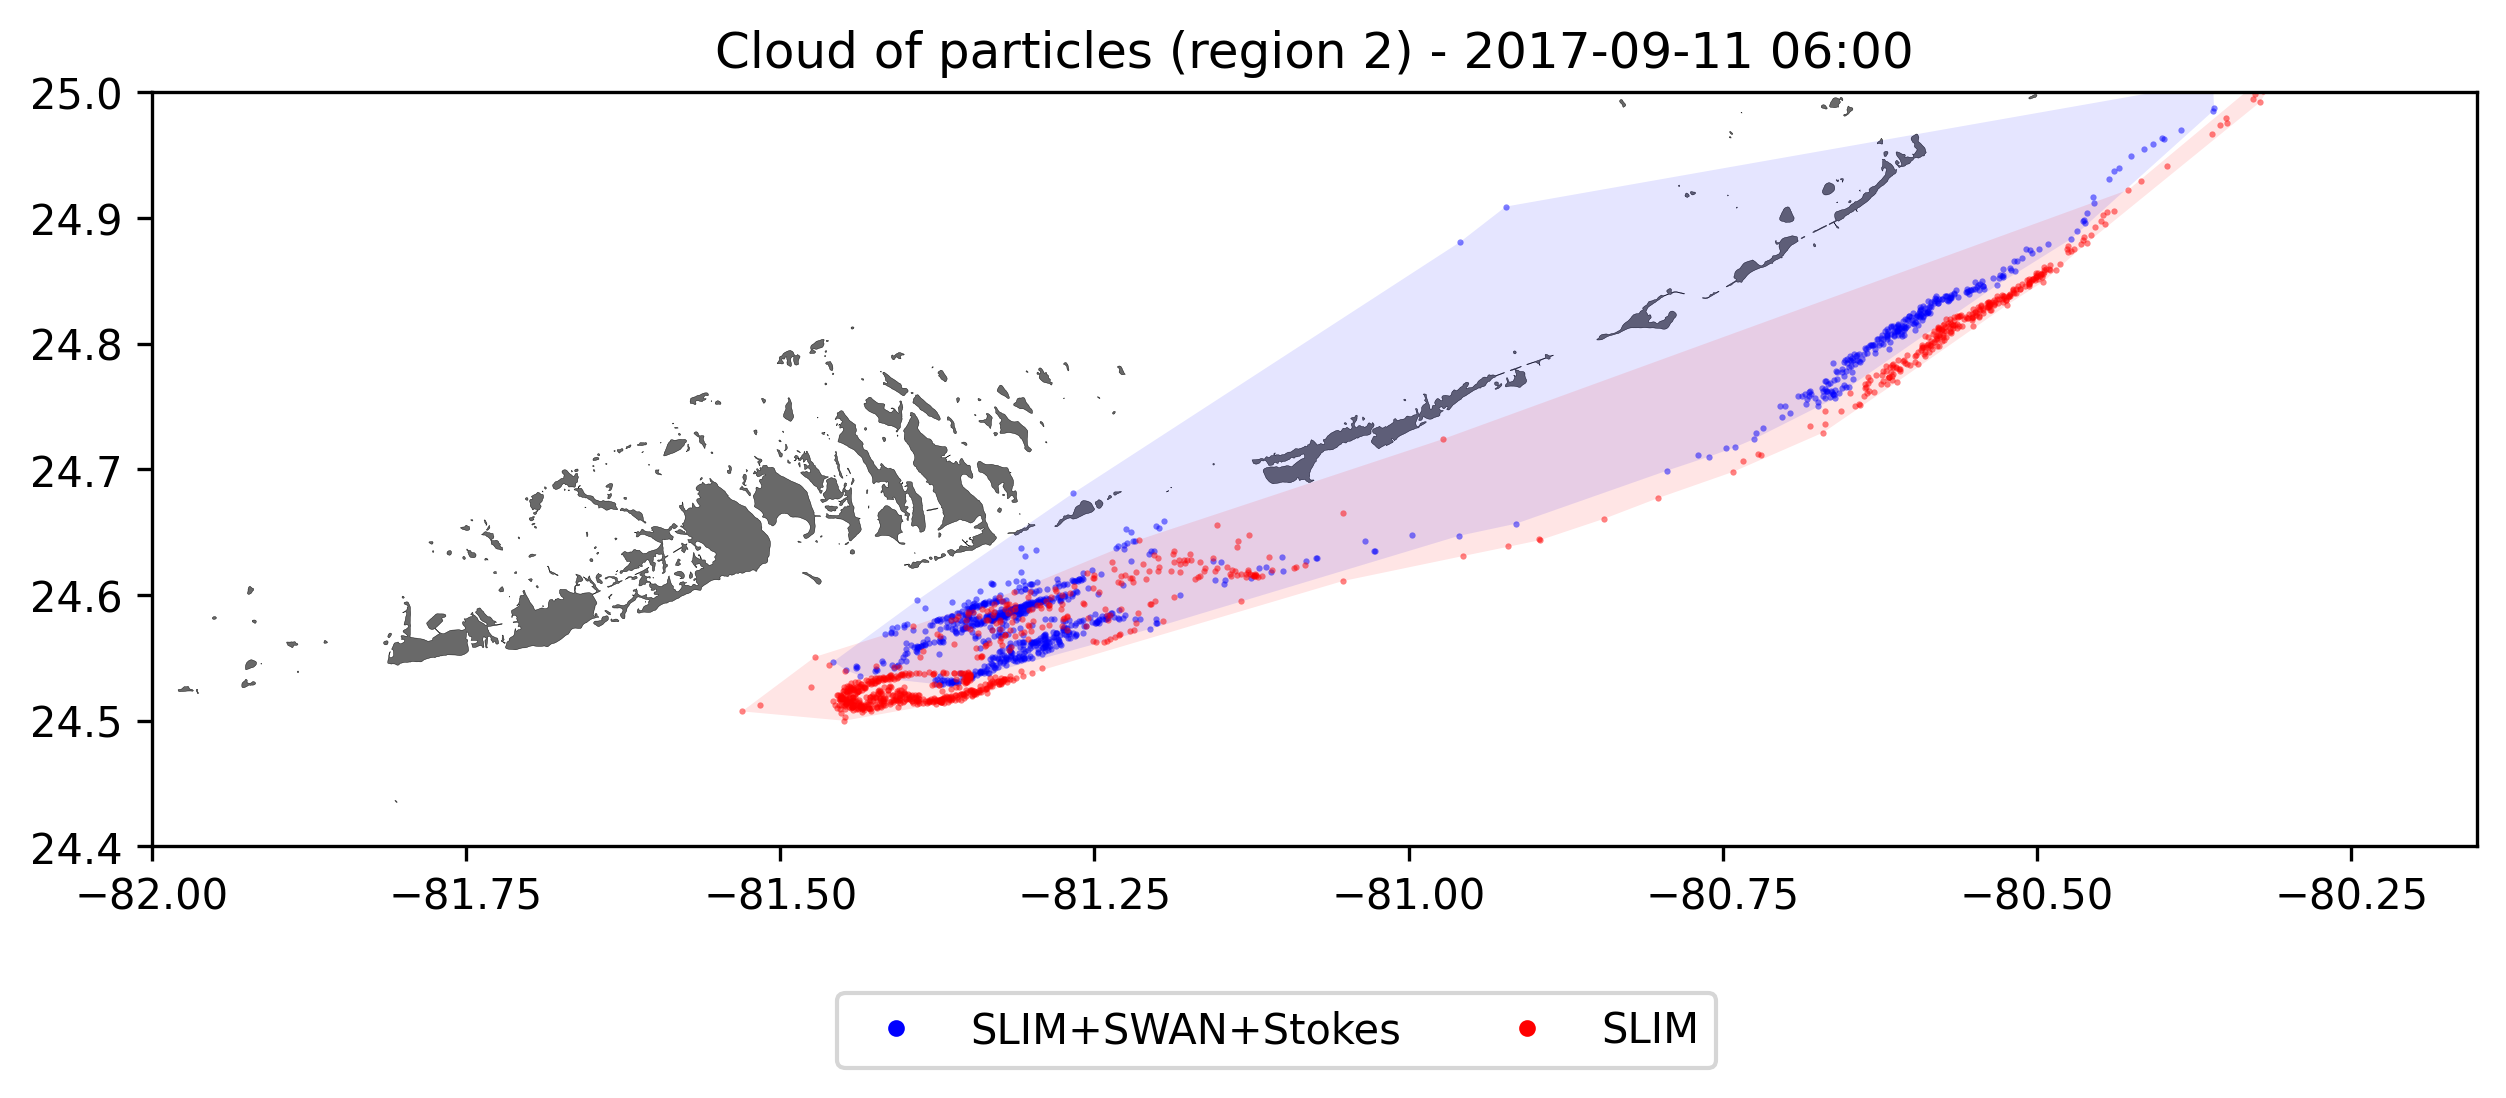
\includegraphics[width=.75\textwidth]{fig/matthieu_ww3.png}
    \caption{Comparison of passive drifters trajectories with SLIM+SWAN+Stokes drift vs. SLIM alone. A snapshot of the positions of the particles released from region 2 is shown after the passage of Irma in the Florida Keys. Particles advected by the currents of the coupled model tend to remain on the shelf while particles advected by SLIM alone are mostly transported along the shelf break}
    \label{fig:diff}
\end{figure}

% === DISCUSSION === %
\section{Discussion and conclusions}

\section*{Conflict of Interest Statement}
The authors declare that the research was conducted in the absence of any commercial or financial relationships that could be construed as a potential conflict of interest.

\section*{Author Contributions}
  
\section*{Funding}

\section*{Acknowledgments}
Computational resources were provided by the Consortium des \'Equipements de Calcul Intensif (\textsc{c\'eci}), funded by the \textsc{f.r.s.-fnrs} under Grant No. 2.5020.11. Thomas Dobbelaere is a PhD student supported by the Fund for Research training in Industry and Agriculture (\textsc{FRIA}/\textsc{FNRS}).

\section*{Supplementary Material}
The Supplementary Material for this article is attached to the submitted document.

% === BIBLIOGRAPHY === %
% \bibliographystyle{frontiersinSCNS_ENG_HUMS} 
\bibliographystyle{apalike}
\bibliography{./biblio.bib}

%%% Make sure to upload the bib file along with the tex file and PDF
%%% Please see the test.bib file for some examples of references

% \appendix
% \section*{Appendix}
% \renewcommand{\thesection}{A}
% \setcounter{figure}{0}
% \renewcommand{\thefigure}{\thesection\arabic{figure}}

\end{document}
